\documentclass[letter,12pt]{article}
\usepackage[letterpaper,right=1in,left=1in,top=1in,bottom=1in]{geometry}
\usepackage{setspace}

\usepackage[utf8]{inputenc}   % allows input of special characters from keyboard (input encoding)
\usepackage[T1]{fontenc}      % what fonts to use when printing characters       (output encoding)
\usepackage{amsmath}          % facilitates writing math formulas and improves the typographical quality of their output
\usepackage[hyphens]{url}     % adds line breaks to long urls
\urlstyle{tt}                 % how urls appear, options tt rm sf and same, see https://mirrors.mit.edu/CTAN/macros/latex/contrib/url/url.pdf
\usepackage[pdftex]{graphicx} % enhanced support for graphics
\usepackage{tikz}             % Easier syntax to draw pgf files (invokes pgf automatically)
\usetikzlibrary{arrows}

\usepackage{mathptmx}           % set font type to Times
\usepackage[scaled=.90]{helvet} % set font type to Times (Helvetica for some special characters)
\usepackage{courier}            % set font type to Times (Courier for other special characters)

\usepackage[longnamesfirst, sort]{natbib}\bibpunct[]{(}{)}{,}{a}{}{;} % handles biblio and references 

\usepackage{rotating}         % sideway tables and figures that take a full page
\usepackage{caption}          % allows multipage figures and tables with same caption (\ContinuedFloat)

\usepackage{dcolumn}          % needed for apsrtable and stargazer tables from R to compile
\usepackage{arydshln}         % dashed lines in tables (hdashline, cdashline{3-4}, 
                              %see http://tex.stackexchange.com/questions/20140/can-a-table-include-a-horizontal-dashed-line)
                              % must be loaded AFTER dcolumn, 
                              %see http://tex.stackexchange.com/questions/12672/which-tabular-packages-do-which-tasks-and-which-packages-conflict


\newcommand{\mc}{\multicolumn}

%% TO ADD NOTES IN TEXT, PUT % BEFORE THE ONE YOU WANT DISABLED
%\usepackage[disable]{todonotes}                            % no show
\usepackage[colorinlistoftodos, textsize=small]{todonotes} % show notes
\newcommand{\emm}[1]{\todo[color=red!15, inline]{\textbf{Eric:} #1}}

%% \usepackage{xr} % allows cross-ref to other file
%% \externaldocument{urge15appendix}

%% %for submission: sends figs, tables, and footnotes to last pages
%% \RequirePackage[nomarkers,nolists]{endfloat}     % sends tables and figures to the end
%% \RequirePackage{endnotes}                        % turns fn into endnotes; place \listofendnotes where you want 
%%                                                  %the endnotes to appear (it must be after the last endnote).
%% \let\footnote=\endnote
%% \newcommand{\listofendnotes}{
%%    \begingroup
%%    \parindent 0pt
%%    \parskip 2ex
%%    \def\enotesize{\normalsize}
%%    \theendnotes
%%    \endgroup
%% }

%% % for submission: drop page numbers when producing title page
%% \pagenumbering{gobble} % Remove page numbers (and reset to 1)
%% \pagenumbering{arabic}% Arabic page numbers (and reset to 1)

\setcitestyle{citesep={;}}

\usepackage{hyperref}

\usepackage{bigfoot}  %% allows the use of \verb command within footnotes

\begin{document}

\title{The Geography of Electoral History: A Dataset of Recent Mexican Election Returns and Quantities of Analytical Interest}
\author{Eric Magar \\ ITAM}
\date{\today}
\maketitle

\noindent The advent of competition in Mexican politics produced a wealth of government data for the analysis of public policy and politics. Data is distributed at the municipal level and smaller geographic units of aggregation (such as census tracts or similar levels), and in some cases at the individual level. This has sprawned fertile areas of new research in education \citep{hoyos.etal.Enlace.2012}, public health \citep{king.etal.segPop.2007, imai.king.nall.segPop.2009}, poverty relief \citep{diaz-estevez-magaloni-Poverty-book.2016, molinar.weldon.1994}, legislative politics \citep{rosas.langston.2011, cantuDesposatoMagar.MxRcv.2014}, and electoral regulation \citep{estevez.magar.rosas.2008}, to name a few.

1952--1967
1965--1976

This paper's focus are vote returns. Electoral data has been distributed for much longer than the information discussed above. It is also better-known and has received a good deal of attention since seminal studies of the PRI's support bases in the states in federal elections of the 1950s and 1960s \citep{ames.1970} and the correlation of modernization measures ant voting and turnout in federal districts between 1965 and 1976 \citep{lehr.1985}. This paper describes a repository...

Some of the distributed data is elementary and available elsewhere, such as the number of valid votes cast for parties in congressional races since 1991 in single-member districts, in municipalities, and in sub-municipal units of aggregation.   shares by party and their change since last election) at the municipal and sub-municipal levels. Offers a cross-section time-series of dip fed returns at two levels of aggregation: municipalities and secciones electorales. 

More abstract

from blog

This note presents, discusses, and distributes statistics (available \href{https://github.com/emagar/mxDistritos}{here}) of party performance in Mexico's competitive era. I elaborate two quantities of interest: *voting forecasts* based on recent electoral history and measures of parties' *core support*. The procedure produces summary measures of recent electoral history in relatively small geographic units, municipalities ($N \approx 2500$) and /secciones electorales/ ($N \approx 66000$) throughout Mexico. I apply the methodology to four federal congressional elections between 2009 and 2018 (I will soon apply it to municipal races too), using results since 1994 as historical input.

The note starts by showing the statistics in action to get a glimpse of their descriptive and analytic potential. By summarizing recent electoral history and its geography, the quantities offer a scenic view of a critical aspect of contemporary Mexican politics. 

Later sections offer methodological detail on the estimation of these quantities of interest and are increasingly technical. 

\section{Municipal governments}
\subsection{Policy making authority}
Mexico's 2,477 (as of January 2025) municipios or municipio-equivalents, into which 31 states and Mexico City are subdivided, are the bottom tier of elected governments. Municipal governments have constitutional authority over community police, zoning and construction permits, water supply, sewerage and waste disposal, street lighting, pavement, and park management, and regulate public markets, slaughterhouses, and cemeteries. They appoint municipal staff and subcontract personnel to carry these responsibilities, key sources of patronnage in a spoils system, making them links of potential importance to political communities in the maintenance of state and national parties \citep{key.1964, sorauf.1959}. 

Municipalities have authority to collect property taxes and fees from public services. State capacity is heterogeneous \citep{garfias.state.cap.2018}, many municipalities, especially in rural Mexico, remain fiscally unorganized and obtain the lion's share of their financial resources from federal revenue sharing and earmarked federal investments \citep{diaz.cayeros.2006, figueroa-mansur-itam.2024}. 

\subsection{Government structure}
Municipal authority is vested in the \emph{Ayuntamiento}, a popularly-elected board deciding by majority rule \citep{robles-mtz.Municipio.2009}. A municipal council (\emph{cabildo}) and a mayor (\emph{presidente municipal} or \emph{primer regidor}) make up the Ayuntamiento. The mayor is executive officer, presides council sessions with voice and the tie-breaking vote, and holds variable municipal appointment powers. Councils, variable in size depending on population, are made up of (1) ranked \emph{regidores} (also called \emph{concejales}), who propose and vote municipal policy through edicts and rulebooks, and (2) possibly one or more \emph{síndicos}, officers in charge of the Treasury and the municipio's legal representation. Where present,\footnote{One state at least \citep[Sinaloa, see][]{rmz-millan.2000} has no síndicos.} síndicos can be elected officers, or council-appointed from among regidores. Municipalities have no judicial power. States do.

Mexico City has a special status. Before 1997, the mayor of the Federal District was a presidential appointee, who would in turn appoint delegates for the city's 16 administrative jurisdictions (called \emph{delegaciones}). A decentralizing reform made all these elected offices in 1997. The Federal District did not, however, gain status as a state, and delegations remained as quasi-municipalities with an elected executive with no fiscal powers (taxation remains in the hands of the city executive) and no elected council. The city further reformed in 2016, adding a council to the quasi-municipalities (now called \emph{alcaldías}) and dropping the name Federal District, becoming simply Mexico City \citep{rabell.2017}.

\subsection{Modal electoral institutions}
Presidents and síndicos (where elected) are elected by plurality. Regidores are elected in two groups (of variable sizes across states), one group by plurality, the other by proportional representation.\footnote{As of 2010, the mean Ayuntamiento had two-thirds of majority seats, with considerable variance. Guanajuato's municipalities, the lowest, had 20 percent. Tabasco's, the highest, had 81 percent. See \citet[][:14]{gil.2010}.} 

Municipal officers are elected in fused tickets. Voters have a single vote, which they cast for a list of candidates including a municipal president on top, ranked regidores, and possibly síndicos. The vote is fused as it simultaneously affects the vote totals of candidates running for different offices \citep[see ][:42]{cox.1997}: the presidency, plurality regidores, and síndicos (where applicable) are allocated to the most voted list. Remaining regidores are distributed to lists proportionally. Split ticket voting is therefore not technically possible.

\subsection{Exceptional electoral institutions}
Two notable exceptions are Chihuahua since 1998 and Nayarit since 2008. Chihuahua's voters have two votes, one to elect the síndico by plurality, another for the remaining municipal officers as described above. This makes split ticket voting possible. 

Nayarit's voters also have dual votes. One vote elects a president and the municipal síndicos by plurality from fused tickets in municipio-wide elections. Another vote elects plurality regidores in single-member districts (municipios are subdivided into districts called \emph{demarcaciones} for the purpose). These other votes are then pooled in a secondary district (the whole municipio) to distribute proportional representation regidores.

\subsection{Term limits}
Municipal governments have three-year terms.\footnote{Four-year terms were found in Coahuila between 2005 and 2016, in Hidalgo since 2016, and in Veracruz between 2013 and 2024. State electoral calendars changed numerous times in the period, exceptionally distorting three-year terms slightly. See \citet{magarInstReel.2017} and \url{https://github.com/emagar/calendarioReeleccion}.} Up to 2018, all were single-term limited, like elected officeholders nationwide since the 1930s. Reform in 2014 let states opt for two-term limits in their municipalities. All states bar Hidalgo did so, the reform kicking off in 2018 in twenty-three states. Ayuntamiento incumbents in the other eight reforming states have been able run for consecutive reelection gradually since. The last will be Veracruz's 212 municipalities in 2025.

Reelection could produce a seismic shift in municipal politics. Six consecutive years in office falls short of qualifying as the long run, but extending Ayuntamientos' time horizons up from just three years should encourage more enterprising policy. More fundamentally, the need to win reelection should encourage ambitious mayors and regidores to keep their electoral alliances alive and mobilized, nurturing responsiveness \citep{cain.etal.1987, jacobson.kernell.1983, cox.mccubbins.1986}.

The removal of single-term limits was surprising given the Mexican elite's anti-reelection rhetoric and might well prove short-lived. Morena, the new partisan Goliath since 2018, has repeatedly voiced determination to reinstate single terms across the board. Regardless, the reform offers an interesting laboratory to study institutional change.   

\subsection{Usos y costumbres}
eric esto falta: preguntarle a Federico dónde se estudia el origen de los 570 municipios.

Oaxaca has 570 municipalities, almost one out of four nationwide. Their origin is colonial, Antequera diffusing ethno-linguistic tensions by creating tiny (in both size and population) majority-minority municipalities \citep{elizarraras.2002}. 

These amount to much fewer formal powers than local goverments in other systems. Mexican municipalities have no jurisdiction over public education and health, lack authority to collect other taxes, and must negotiate some fiscal resources with the state government, who may be tempted to bias redistribution of revenue sharing to municipalities \citep{timmons.broid.2013} 

Still, the institutional heterogeneity and variable socio-economic conditions make them very interesting for social science. 

But interest in Mexico's municipal government has nonetheless grown

But, with much heterogeneity, municipal governments grew in importance between 1990 and 2010. Percent of public spending they exert... making them, and the variance they manifest, attractive areas for the study of politics and policy. 

\section{Municipal election data}
This research note introduces a dataset of municipal election vote returns in recent decades. The dataset is distributed in a repository, publicly available at \url{https://github.com/emagar/elecRetrns}, that also includes returns to gubernatorial races and federal elections at different levels of aggregation.\footnote{The \emph{Recent Mexican Election Vote Returns} repository is publicly available at \url{https://github.com/emagar/elecRetrns}.} 

The municipal election dataset has been under construction for some time. The original seed for the 1970s and 1980s was compiled by \citet{molinar.1991a} from official vote returns by the Interior Ministry's Registro Nacional de Electores. The primary source was systematized by \citet{magar.1994} for northern Mexico and then by \citet{varela.2004} nationwide. Data from the 1990s onwards was compiled from the new state election regulators, who more or less routinely report vote returns since. When that was not the case, other sources were consulted, most notably \citet{revista.voz.y.voto} and \citet{cede.uam.izt}.

The unit of observation is the municipality, reporting the votes each party or electoral coalition won in periodic elections.

Data is available in a handful of states since the early 1970s, but the full cross-sectional time-series in the dataset really begins in the 1979--1981 trienium. This period, inaugurated by a major federal electoral reform (the LFOPPE), lowered legal entry barriers and adopted a more proportional electoral formula in Congress \citep[:116]{molinar.1991a}. As a result, half a dozen new parties entered the electoral arena. Table \ref{T:coverage} summarizes data coverage by state, reporting the number of municipalities (which increased over the years in most states)\footnote{File \verb|ancillary/mun.yrs.csv| in the repository reports the full listing of municipalities in each election cycle with available municipal election returns. And file \verb|ancillary/new-mun-parents-1989on.csv| reports the parent municipalities from which the new units seceded. State abbreviations are different than those used by Mexican government agencies, some were slightly altered so that sorting them in a standard spreadsheet retains the actual alphabetical ordering of the states (e.g. Guanajuato and Guerrero are abbreviated gua and gue instead of the official gto and gro).} Mexico City's populous units are included in the data despite their special status.

\begin{table}
\resizebox{.8\textwidth}{!}{
    \begin{tabular}{rlrc}
      & State (abbreviation)                        & Number of municipalities & Years      \\ \hline
      1  & Aguascalientes                 (ags)        &      9--11           & 1977--2024 \\
      2  & Baja California                (bc)         &       4--7           & 1971--2024 \\
      3  & Baja California Sur            (bcs)        &       3--5           & 1974--2024 \\
      4  & Campeche                       (cam)        &      8--13           & 1979--2024 \\ \hdashline
      5  & Coahuila                       (coa)        &         38           & 1978--2024 \\
      6  & Colima                         (col)        &         10           & 1976--2024 \\
      7  & Chiapas$^\dagger$               (cps)        &   110--126           & 1976--2024 \\
      8  & Chihuahua                      (cua)        &         67           & 1974--2024 \\ \hdashline
      9  & Distrito Federal/Mexico City$^\ddagger$ (df) &         16           & 1997--2024 \\
      10 & Durango                        (dgo)        &     38--39           & 1971--2024 \\
      11 & Guanajuato                     (gua)        &         46           & 1979--2024 \\
      12 & Guerrero$^\dagger$              (gue)        &     75--85           & 1977--2024 \\ \hdashline
      13 & Hidalgo                        (hgo)        &         84           & 1981--2024 \\
      14 & Jalisco                        (jal)        &   124--125           & 1976--2024 \\
      15 & México                         (mex)        &   121--125           & 1978--2024 \\
      16 & Michoacán$^\dagger$             (mic)        &        113           & 1977--2024 \\ \hdashline
      17 & Morelos$^\dagger$               (mor)        &     33--36           & 1976--2024 \\
      18 & Nayarit                        (nay)        &     19--20           & 1972--2024 \\
      19 & Nuevo León                     (nl)         &         51           & 1973--2024 \\
      20 & Oaxaca$^\dagger$                (oax)        &        570           & 1977--2024 \\ \hdashline
      21 & Puebla                         (pue)        &        217           & 1980--2024 \\
      22 & Querétaro                      (que)        &         18           & 1973--2024 \\
      23 & Quintana Roo                   (qui)        &      7--11           & 1978--2024 \\
      24 & San Luis Potosí                (san)        &     56--58           & 1970--2024 \\ \hdashline
      25 & Sinaloa                        (sin)        &     17--20           & 1971--2024 \\
      26 & Sonora                         (son)        &     69--72           & 1976--2024 \\
      27 & Tabasco                        (tab)        &         17           & 1976--2024 \\
      28 & Tamaulipas                     (tam)        &         43           & 1971--2024 \\ \hdashline
      29 & Tlaxcala                       (tla)        &      44-60           & 1979--2024 \\
      30 & Veracruz                       (ver)        &   203--212           & 1976--2024 \\
      31 & Yucatán                        (yuc)        &        106           & 1981--2024 \\
      32 & Zacatecas                      (zac)        &     56--58           & 1970--2024 \\ \hline
        & \mc{1}{l}{Municipalities nationwide by election cycle} & 2375--2477 & 1970--2024 \\
    \end{tabular}
}
\caption{Coverage of the election returns data at the municipal level. $\dagger$  Reform in these states withdrew so-called `usos y costumbres' municipalities from the periodic electoral process: one municipality in Chiapas since 2021, one in Guerrero since 2018 and another since 2024, one in Michoacán since 2011, three in Morelos since 2021, and between 412 and 418 in Oaxaca since 1995. $\ddagger$ Administrative jurisdictions in the Federal District became elected offices since 1997, see the text for details.}\label{T:coverage}
\end{table}

Municipal election vote returns are distributed as a large cross-section time-series. Data is stored as text in \verb|csv| format (comma separated values), easily accessible for inspection with spreadsheet software such as Microsoft Excel or open-source Libreoffice Calc.\footnote{Text is stored in UTF-8 character encryption. Care has been taken to drop most Latin American special characters, such as accented vowels, from text strings. The letter \~N remains, and may appear as a garbled character in machines with other default encryption systems. See \url{https://docs.python.org/3/howto/unicode.html} for a primer on character encryption.} In the resulting data matrix, each row is a municipality in a given electoral year. Columns are data fields, including unit identifiers (the municipality's name, state, census bureau ID, an so forth), the election date, and the vote total that each party or coalition won.\footnote{The repository's \verb|README.md| file includes a detailed codebook describing what is in each spreadsheet column/field.} Also included is the vote total, to compute vote shares, and the number of eligible voters in the municipal election (the \emph{lista nominal}), to compute turnout rates.  

Vote returns appear in column pairs for each party or coalition: columns \verb|v01, v02, ...| report raw vote totals, columns \verb|l01, l02, ...| the label of the party or coalition the votes belong to. Figure \ref{F:scrn} offers a glimpse for the state of Baja California's five municipalities over three election cycles. In Ensenada for $\texttt{yr} = 1998$, that $\texttt{v01} = 30660$, $\texttt{l01} = \texttt{pan}$, $\texttt{v02} = 31951$, and $\texttt{l02} = \texttt{pri}$ reveals that the National Action Party (PAN) won 30,660 votes, not far from but below the PRI's 31,951 votes. The vote/label column pairs accommodate state party system heterogeneity over four decades of high mutability, and ephemerous electoral coalitions (as in Baja California in 2001 and in 2004) in a relatively small number of columns. The trade-off is that compiling one party's votes for each of a state-year's municipalities often requires some manipulation, as it may not appear in the same column. 

\begin{figure}
  \centering
  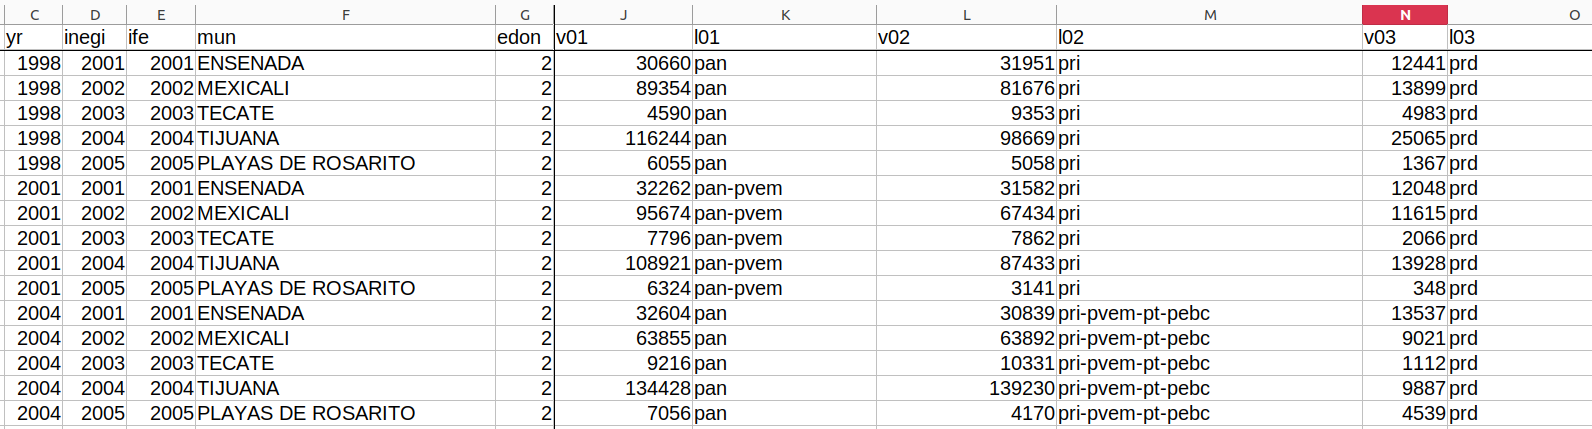
\includegraphics[width=\columnwidth]{pics/eg-spreadsheet-columns.png}
  \caption{Screenshot with a sample of the data organization}\label{F:scrn}
\end{figure}  

The data is stored in three separate files with the same observations: one has raw votes as reported in the primary source; one systematically aggregates coalition votes; one splits the votes that each coalesced party contributed to the coalition total.\footnote{Files are \verb|aymu1970-on.csv|, \verb|aymu1970-on.coalAgg.csv|, and \verb|aymu1970-on.coalSplit.csv| respectively. Mexican election law distinguishes two forms of pre-election coalitions that parties may choose from: joint candidacies and coalitions proper. Voters can cast a vote for any joint-candidate-nominating party (or combinations of them), which are then added to determine the winning candidate, but can only cast a vote for the team as a whole in coalitions proper---hence the need for three municipal vote files. These subtleties have effects in public party finance mostly, but substantially complicate voting studies as scholars need to decide how to handle coalitions. In coalitions proper, and whenever the primary source does not offer the coalesced-parties vote breakdown, one artifical vote is added to the raw file, itself split among these parties to keep track of relative contributions (one esample is Baja California in 2007).} Banned until the mid-1980s at the local level, and rarely authorized up to the mid-1990s, coalitions have since become a staple of Mexican elections. Table \ref{T:coal} reports the the mean number of coalitions per municipal election and their coalitional profile in each federal election cycle. The mean number of coalitions surpassed one by 2006--09, up from 0.29 six years before, and rose to a maximum 1.85 in 2018. It has declined since. Other columns in the table reveal the dynamic: in a first moment between 2000 and 2009, at least one major party, and increasingly two major parties would team up with minor parties (`major-minor' arrangements) to gain an edge in municipal races. A second moment in 2009 and 2012 inaugurated frequent `double-major' races, PAN and PRD forging anti-PRI coalitions in over a fifth of municipalities. A third moment came with Morena's foray into the party system, forcing frequent regroupments of erstwhile rivals PAN, PRI, and PRD (`triple-major' coalitions)) that reduced the number of coalitions per municipality by widening their scope. 

\begin{table}
\resizebox{\textwidth}{!}{
\begin{tabular}{r|c|rrrrrrrrrr}
       & (Mean co-  &      & One          & Two        & Three      &               & Double-major  & Double-major      &             & Triple-major   &       \\
 Cycle & alitions)  &  None&  major-minor & major-minor& major-minor&   Double-major& \& major-minor& \& two major-minor& Triple-major&  \& major-minor& Total \\
       &            &      &              &            &            &               &               &                   &             &                &       \\ [-1.8ex] \hline
       &            &      &              &            &            &               &               &                   &             &                &        \\[-1.8ex] 
       &            &      &              &            &            &               &               &                   &             &                &       \\ [-1.8ex] 
 1979& (0.00)& 100.0&   ---&    ---&    ---&    ---&       ---&         ---&  ---&       ---& 100.0\\
 1982& (0.00)& 100.0&   ---&    ---&    ---&    ---&       ---&         ---&  ---&       ---& 100.0\\
 1985& (0.00)& 100.0&   ---&    ---&    ---&    ---&       ---&         ---&  ---&       ---& 100.0\\
 1988& (0.05)&  93.9&   6.1&    ---&    ---&    ---&       ---&         ---&  ---&       ---& 100.0\\ \hdashline
 1991& (0.01)&  98.6&   1.3&    ---&    ---&    ---&       ---&         ---&  ---&       ---& 100.0\\
 1994& (0.04)&  99.8&   0.2&    ---&    ---&    ---&       ---&         ---&  ---&       ---& 100.0\\
 1997& (0.03)&  96.4&   2.1&    ---&    ---&    1.5&       ---&         ---&  ---&       ---& 100.0\\
 2000& (0.29)&  77.0&  16.7&    1.8&    ---&    4.0&       0.4&         ---&  ---&       ---& 100.0\\ \hdashline
 2003& (0.64)&  52.8&  29.8&   11.8&    0.4&    1.8&       3.3&         ---&  ---&       ---& 100.0\\
 2006& (1.18)&  20.4&  48.1&   30.2&    0.6&    0.1&       0.7&         ---&  ---&       ---& 100.0\\
 2009& (1.53)&  11.2&  32.3&   14.6&   10.4&    7.7&      23.8&         ---&  ---&       ---& 100.0\\
 2012& (1.38)&   8.6&  50.8&   11.6&    3.6&    3.5&      21.9&         ---&  ---&       ---& 100.0\\ \hdashline
 2015& (1.16)&  24.6&  35.6&   11.0&    0.8&    6.1&      21.8&         ---&  0.2&       ---& 100.0\\
 2018& (1.85)&   6.3&  17.4&   14.7&    7.1&    6.5&      35.0&        12.9&  ---&       ---& 100.0\\
 2021& (1.03)&  26.8&  18.5&    0.2&    ---&   13.0&       9.5&         0.3& 18.2&      13.6& 100.0\\
 2024& (1.17)&  27.2&  11.4&    1.6&    ---&    6.0&      11.2&         0.7& 17.1&      24.8& 100.0\\ 
     &       &      &      &       &       &       &          &            &     &          &      \\ [-1.8ex] 
  \hline \\[-1.8ex] 
\end{tabular}
}
\caption{Coalitional profile frequency by federal election cycle (percentage municipalities). Table considers coalitions where one partner at least was a major party (PAN, PRI, PRD, or Morena), ignoring coalitions involving minor parties only, which were also quite frequent.}\label{T:coal}
\end{table}

Figure \ref{F:vpcts}, which summarizes municipal elections since 1979, adds another descriptive layer. Plot shares PAN PRI PRD Morena Other each year: tiny points, mean and 80band 

\begin{figure}
  \includegraphics[width=\columnwidth]{../../plots/vpct1979-2024.pdf}
  \caption{The evolution of electoral parties in municipal races 1979--2024. Lines are the vote percentage each party won in the median municipality across time (the trend is smoothed for clarity). Each color-coded tiny circle is one individual party's vote percentage in one municipal election (slightly x-jittered for visibility and excluding the residual `others' category).}\label{F:vpcts}
\end{figure}  



Coaliciones and candidatos comunes.

Winners in the incumbents dataset. 

\section{Reelection as insurance policy}
Also discusses another dataset in the repository, incumbents.

\section{The measurement of electoral history}
Also discusses another dataset in the repository, vhats.

\section{Non-fused tickets in Nayarit}
Also discusses another dataset in the repository, nayreg.

Table [[fig:1]] presents two pairs of diagrams for the 2015 (below) and 2018 (above) congressional elections. Each dot represents one municipality, colored according to the winning party, with coordinates in the ternary plot according to the relative votes of the PAN, the PRI, and the left in the federal deputy race (other smaller parties are excluded).\footnote{I must note that, for the left's electoral history (which I arbitrarily call ``Morena'' in the plots and distributed data), I systematically added up the votes of the PRD, PT, and MC up to 2015. I also added Morena's and PES's votes that year. In 2018 the left consisted of Morena, PT, and PES jointly.} 

% \begin{figure}
% \centering
% \caption{Historic expectations and municipal-level vote in two congressional elections}\label{fig:1}
% \begin{tabular}{cc}
%   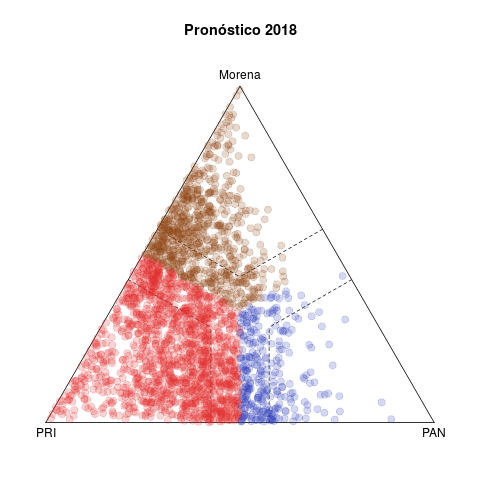
\includegraphics[width=.75\columnwidth]{../assets/img/triplot2018-vhat-mu.png} &
%   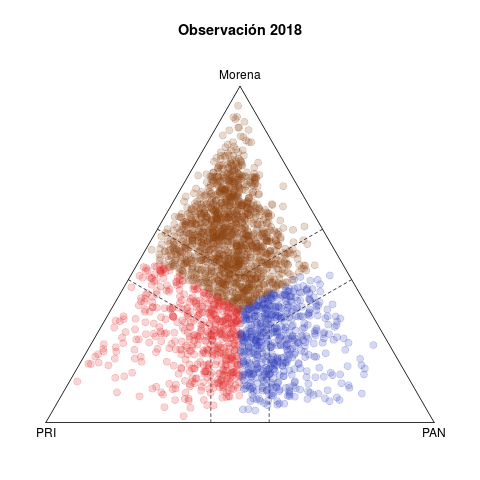
\includegraphics[width=.75\columnwidth]{../assets/img/triplot2018-v-mu.png}    \\
%   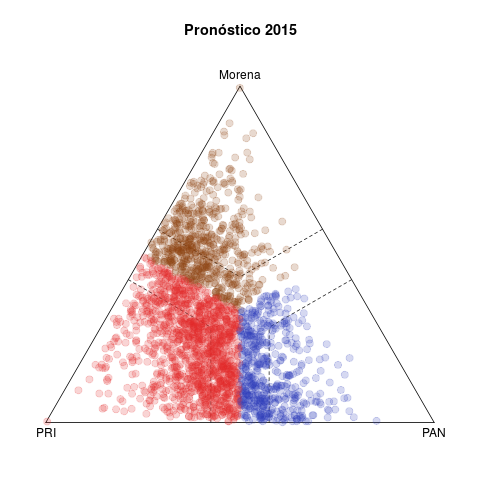
\includegraphics[width=.75\columnwidth]{../assets/img/triplot2015-vhat-mu.png} &
%   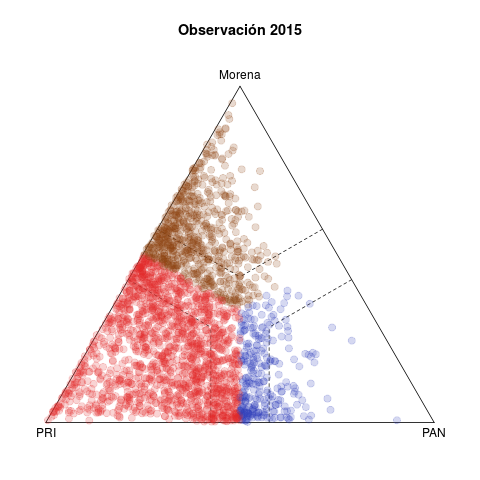
\includegraphics[width=.75\columnwidth]{file:../assets/img/triplot2015-v-mu.png} \\
% \end{tabular}
% \end{figure}

The left side shows the /vote forecasts/. The idea behind this statistic is summarizing the evolution of relative votes in the municipality in five previous elections (2003--2015 in the case of 2018) and using the tendency to project a vote forecast for the current year. Plots in the right side show the actual results observed in both elections.

Three features are noteworthy in 2018. The first is the discrepancy between the left and right plots. Either the model does a poor job forecasting, or 2018 was an extraordinary election. History gave license to expect a comfortable PRI victory, both in the number of municipalities won and in margins of victory. Municipalities outside the dotted bands are won by margins of 15 points or more, and the bulk of secure municipalities are red in the forecast, with Morena in a distant second place. In fact, although a significant number of municipalities migrated towards the PAN, it was Morena who showed a clear advantage. PRI was the underachiever. In contrast, the lower left and right plots reveal fewer differences between them---2015 was a more normal election, the past offering much better grounds to forecast. 

Second, observed municipalities fled the edges and triangle vertices in 2018. Observations in vertices show a party that has no significant challenger. While those on the edges were bipartisan, whether more (inside dotted bands) or less (outside the bands) symmetric. It is also plain in forecasts that only the PAN--Morena edge was expected to be unpopulated. In practice, however, third party vote rarely collapsed to zero, there was much more dis-coordination than in the past. In fact, the intersection of dotted bands appeared denser and more homogeneous in the right than the left diagram. 

Third, the PAN /vs/ left competition was legal tender in 2018. The pattern in competitive municipalities in the last two decades, still visible in the 2015 plots, involved either PRI--PAN or PRI--left rivalries, and rarely PAN--izquierda. It was this pattern that eased electoral alliances between PAN and PRD in sub national races since 2010 that culminated in the Frente they formed in 2018 to nominate a joint presidential candidate. 

% # #+CAPTION: Una elección más característica de la partidocracia
% # #+NAME:   fig:2
% # | file:../assets/img/triplot2015-vhat-mu.png | [[file:../assets/img/triplot2015-v-mu.png]] |


% # #+CAPTION: Grano más fino: las secciones
% # #+NAME:   fig:3
% # | file:../assets/img/triplot2015-v-se.png | [[file:../assets/img/triplot2018-v-se.png]] |

Plots in Table [[fig:4]] report /secciones electorales/ and therefore offer much finer-grained than the previous portraits. They introduce the other quantity of interest in this note: parties' /core support/. The idea behind this statistic is measuring the size of the group that has historically supported the party consistently, in good but also in bad years. 

% #+CAPTION: Support core and party performance in 2018
% #+NAME:   fig:4
% | file:../assets/img/resid-pan-2018-vs-pan-core-se.png | [[file:../assets/img/resid-morena-2018-vs-morena-core-se.png]] | file:../assets/img/resid-pri-2018-vs-pri-core-se.png |

The horizontal axis in each plot measures the size of party core support groups as a proportion of the /sección/'s electorate. The PRI enjoyed a clear edge over the rest of the parties in the period, with sizable cores in /all/ secciones nationwide. The distributions of the PAN and the left, in contrast, appear concentrated towards the zero---they have relatively few secciones with some unconditional support. 

The vertical axis reports the three parties' performance in 2018 (the difference between the observed vote and the forecast). Positive values indicate that the party excelled expectations in the /sección/, negative ones that it under-performed it expectation. The PRI's electoral disaster appears all too clearly in the red plot. There were a few secciones with positive performance, but the density concentrates massively below the horizontal zero line, something that Table [[fig:1]] had hinted. What is truly remarkable is that the dismal performance is directly proportional to the size of the PRI core. President Peña and candidate Meade achieved what seemed, if not impossible, extremely improbable: they alienated the PRI's unconditional voters in 2018. The PAN and the left met expectations in secciones where they have enjoyed with groups of support. Both (especially Morena) over-achieved where they lack important cores, taking away PRI voters. 

The note elaborates how statistics were prepared (replication code can be found [[https://github.com/emagar/mxDistritos/code/elec-data-for-maps.r][here]]).

% # [[file:https://github.com/emagar/elecRetrns/raw/master/graph/nytAmloPlusAnayaPlusMeadeNegPenaWon.svg]]

% # #+CAPTION: PAN
% # #+NAME:   fig:6
% # #+ATTR_HTML: style="float:right;"
% # #+ATTR_HTML: :width 50%
% # [[file:../assets/img/resid-pan-2018-vs-pan-core-se.png]]

* First differences
One common approach to study electoral change is through first differences. Denoting $v_t$ the party's vote share in the municipality or the /sección/, in period $t$, the first difference is simply $d_t = v_t - v_{t-1}$. 

$d_t$ is an intuitive quantity, showing the sign and magnitude of change from one election to the next. But, precisely because it compares pairs of consecutive elections only, it misses more dynamic processes in the units. One example, well documented by electoral sociology, is the regression to the mean \citep{campbell.1991,segovia.1979}. Its detection requires observing the unit through at least three consecutive periods to verify contrary signs in $d_{t+1}$ and $d_t$. The study of secular change in the Mexican party system in the last quarter of century calls for deeper historical perspective. 

(First differences appear in the fields ~d.pan~, ~d.pri~, and ~d.morena~ in the distributed data.)

* The recent linear tendency
One way of adopting it is with /vote forecasting/ from tendencies discernible in the previous five congressional races \citep{magar.gubCoatMx.2012}. I summarize the central tendency of the recent historical vote by means of linear estimation in time, fitting a straight line for each year analyzed and each party in the municipality or /sección electoral/. 

The slope of the fitted line (the tendency) serves to extrapolate the party's electoral support to the future. For instance, to get the vote share that the recent past predicts for a party in unit $u$ for 2018, I estimate the following equation 

\begin{equation}
v_{ut} = a_u + b_u \times t + \text{error}_{ut}, \; t = 2003, \ldots, 2015
\end{equation}\label{ts-eq}

that I then use to predict $\hat{v}_{u2018} = \hat{a}_u + \hat{b}_u \times 2018$. This is an out-of-sample prediction of the party's vote share, it can be compared to the party's actual vote share in 2018 to gauge whether or not the unit approximates the historical record. For the 2015 forecast the sample shifts one period to become $t = 2000, \ldots, 2012$, and so on an so forth for previous years. I distribute forecasts for 2009, 2012, 2015, and 2018, which involved fitting about 10 thousand municipal regressions and more than 250 thousand sección-level.

(Vote forecasts appear in the fields ~vhat.pan~, ~vhat.pri~, and ~vhat.morena~ of the distributed data.)

* The party's support core
The other historical statistic is the parties' core support in the unit. Its definition stems from classifying voters in three categories: (1) support groups, that in the past have consistently supported the party; (2) opposition groups, that have consistently supported another party; and (3) swing groups, that have neither consistently supported nor consistently opposed the party \citep{cox.mccubbins.1986}. The party core consists of the support groups. 

I use the procedure by Díaz Cayeros /et al/. (2016) to estimate this core. If $\bar{v}_t$ denotes the party's mean support across all units in period $t$,\footnote{The analyzed unit $u$ should be dropped from period $t$'s mean in order to not include the dependent variable in the right side of equation \ref{ts-eq}. I do not drop it due to the large number of municipal or seccional units (each contributing a fraction to the mean) and the use of vote shares (so large units are watered down): this refinement's impact should be negligible in each mean value.} for each party in each unit I fit

\begin{equation}
v_{ut} = \alpha_u + \beta_u \times \bar{v}_t + \text{error}_{ut}, \; t = 1994, \ldots, 2018.
\end{equation}\label{alpha-eq}

$\beta_u$ measures the effect that national party tides have on the party's vote in unit $u$. For instance, $\hat{\beta}_u=1$ estimates that for every percentage point that the party wins or loses nationally in year $t$, it also wins or loses one percentage point in the unit; $\hat{\beta}_u=0$, on the other hand, would indicate the unit's full isolation form national swings. It is therefore a measure of party volatility in the municipality or /sección/ (analogous to \href{https://www.investopedia.com/terms/v/volatility.asp}{"beta volatility"} in the financial literature). 

The $\alpha$ coefficient estimates the core size: expected support in unit $u$ in the hypothetical case that the party receives no vote at the national level. For instance, $\hat{\alpha}=.4$ would indicate that, in the starkest of scenarios, 40% of the electorate in the municipality is unconditional to the party---which would indeed be a core of substantial size.

A critique that can be anticipated towards this measure of the party's support core is its extreme counter-factual nature \citep{king.zeng.counterfactuals2006pa}. It deserves rigorous scrutiny, something I plan doing in the near future. 

(The parties' core support appears in the fields ~alphahat.pan~, ~alphahat.pri~, and ~alphahat.morena~ of the distributed data. Party volatility in ~betahat.pan~, ~betahat.pri~, and ~betahat.morena~.)

* Compositional variables
I close with an important feature of the model specifications, associated with the \emph{compositional} nature of electoral returns. Compositional variable are quantitative descriptions of the parts of a whole. They therefore have two characteristics: (1) they are proportions that (2) add up to unity.\footnote{Formally, the compositional are random variables subject to two constraints: 
$0 \leq v_p \leq 1 \; \forall \; p \in P \; \; and \; \; \sum_P v_p = 1.$.} 

When estimating parties separately, the challenge of equations 1 and 2 is to avoid forecasting vote shares less than zero or greater than one; and that the sum of party forecasts equals 1. To achieve this, \citet{aitchison.1986} proposes substituting vote shares by log-ratios in the analysis. Arbitrarily setting the PRI as the reference party, define party $p$'s vote relative to the PRI as 

$r_p = \frac{v_p}{v_{\text{pri}}}.$

A value $r_p=1$ would indicate a tie between the party and the PRI, while $r_p>1$ that it finished ahead of the PRI in the proportion that the value reveals. 

Thus, equation 1 is re-specified as

$\ln r_{put} = a + b \times t + \text{error}$

y equation 2 as

$\ln r_{put} = \alpha + \beta \times \bar{r}_{pt} + \text{error}.$

Applying the natural logarithm attenuates the effect of extreme values of the regressor on the dependent variable, similar as a logit regression would. Models fitting was done with ordinary least squares. 

Coefficient estimates requires transformation to collect party vote shares. Illustrating with a three-party caste, it is trivial that 

\begin{equation}
\hat{v}_p = \frac{\hat{r}_p}{1 + \hat{r}_{\text{pan}} + \hat{r}_{\text{morena}}} \; \text{and} \;
\hat{v}_{\text{pri}} = \frac{1}{1 + \hat{r}_{\text{pan}} + \hat{r}_{\text{morena}}.}
\end{equation}

%% \begin{equation}
%% \begin{split}
%% v_{\text{pri}} + v_{\text{pan}} + v_{\text{morena}} & = 1 \\
%% v_{\text{pri}} & = 1 - v_{\text{pan}} - v_{\text{morena}} \\
%% 1 & = \frac{1}{v_{\text{pri}}} - \frac{v_{\text{pan}}}{v_{\text{pri}}} - \frac{v_{\text{morena}}}{v_{\text{pri}}} \\
%% \end{split}
%% \end{equation}

These are the quantities that the distributed data report. 


% # Fácil de implementar en R:
% # a = voto partido unidad 1
% # A = voto efec unidad 1
% # N = 3 unidades
% #
% # tengo
% # v.bar = 1/3 * (a/A + b/B + c/C)
% #
% # quiero
% # v.bar.sin.aA = 1/2 * (b/B + c/C)
% #
% # hago
% # 1/3 * (a/A + b/B + c/C) =      v.bar
% #        a/A + b/B + c/C  =  3 * v.bar
% #              b/B + c/C  =  3 * v.bar - a/A
% #       1/2 * (b/B + c/C) = (3 * v.bar - a/A) * 1/2 = v.bar.sin.aA
% #
% # v.bar.sin.aA = (N * v.bar - a/A) * 1/(N-1)



\bibliographystyle{apsr}
\bibliography{/home/eric/Dropbox/mydocs/magar}


\end{document}
